%%% %%%%%%%%%%%%%%%%%%%%%%%%%%%%%%%%%%%%%%%%%%%%%%%%%%%%%%%%%%%%%%%%%%%%%%%%%%%% 

\rawhtml
<a name="production_code_program_synthesis"></a>
\endrawhtml
\subsectional{Generation: Automated Code Synthesis}

%%% %%%%%%%%%%%%%%%%%%%%%%%%%%%%%%%%%%%%%%%%%%%%%%%%%%%%%%%%%%%%%%%%%%%%%%%%%%%% 

Given the title, you might have thought this document would be all about automatic programming, but it's really about human augmentation and human-computer collaboration. Programming is all about representing procedural knowledge in an interpretable form, i.e., executable on some computational substrate. Teaching someone to program or, for that matter, teaching someone to do most anything is also about representing and communicating procedural knowledge in an interpretable form \emdash{} the clearer and more precise the communication the simpler and less knowledgeable the computational substrate.

In this section, we attempt to identify special cases in which it is relatively easy for a human programmer to instruct an AI system how to facilitate the conversion of thoughts conveyed in natural language into working programs. We are not anticipating that we will be able to read minds so much as exploit shared knowledge in order to translate succinct descriptions of desired computations \emdash{} along with an implicit understanding of what constitutes a suitable computational solution \emdash{} into working software possibly with guarantees of its correctness and performance.

How does this perspective inform the discussion in this section? Prior to any training the apprentice comes equipped with a very basic language facility and an innate ability to work with computer programs, but the former is practically useless since the meta-learning controller hasn't been trained and the latter only produces results in the same way that a baby has virtually no control over its limbs and torso. It learns to communicate by reinforcement when it successfully carries out a command from the expert programmer. A built-in training system expedites this process and relieves some of the burden from the programmer by generating synthetic commands that serve to initialize the meta-learning controller allowing the assistant to achieve a basic facility for directly translating natural language commands exercising the integrated development environment.

The apprentice also comes pre-trained with a (semantic) language model trained on a corpus that includes a large vocabulary of practical and technical terms used by programmers in talking about programs and programming. The system has also ingested a large corpus of programs and program fragments written in the language that it will use for writing new programs, resulting in an embedding space that encodes these programs and an encoder decoder translation facility that allows it to read and write programs represented as abstract syntax trees.

%%% %%%%%%%%%%%%%%%%%%%%%%%%%%%%%%%%%%%%%%%%%%%%%%%%%%%%%%%%%%%%%%%%%%%%%%%%%%%% 

\setcounter{figure}{2}

%%% %%%%%%%%%%%%%%%%%%%%%%%%%%%%%%%%%%%%%%%%%%%%%%%%%%%%%%%%%%%%%%%%%%%%%%%%%%%% 

%%% Figure~{\urlh{#fig_CS379C_Final_Project_Gomezetal_Figure_03}{3}}
\rawhtml
<a name="fig_CS379C_Final_Project_Gomezetal_Figure_03"></a>
\endrawhtml
\begin{figure}
%
  \hrule{}
%
  \begin{center}
    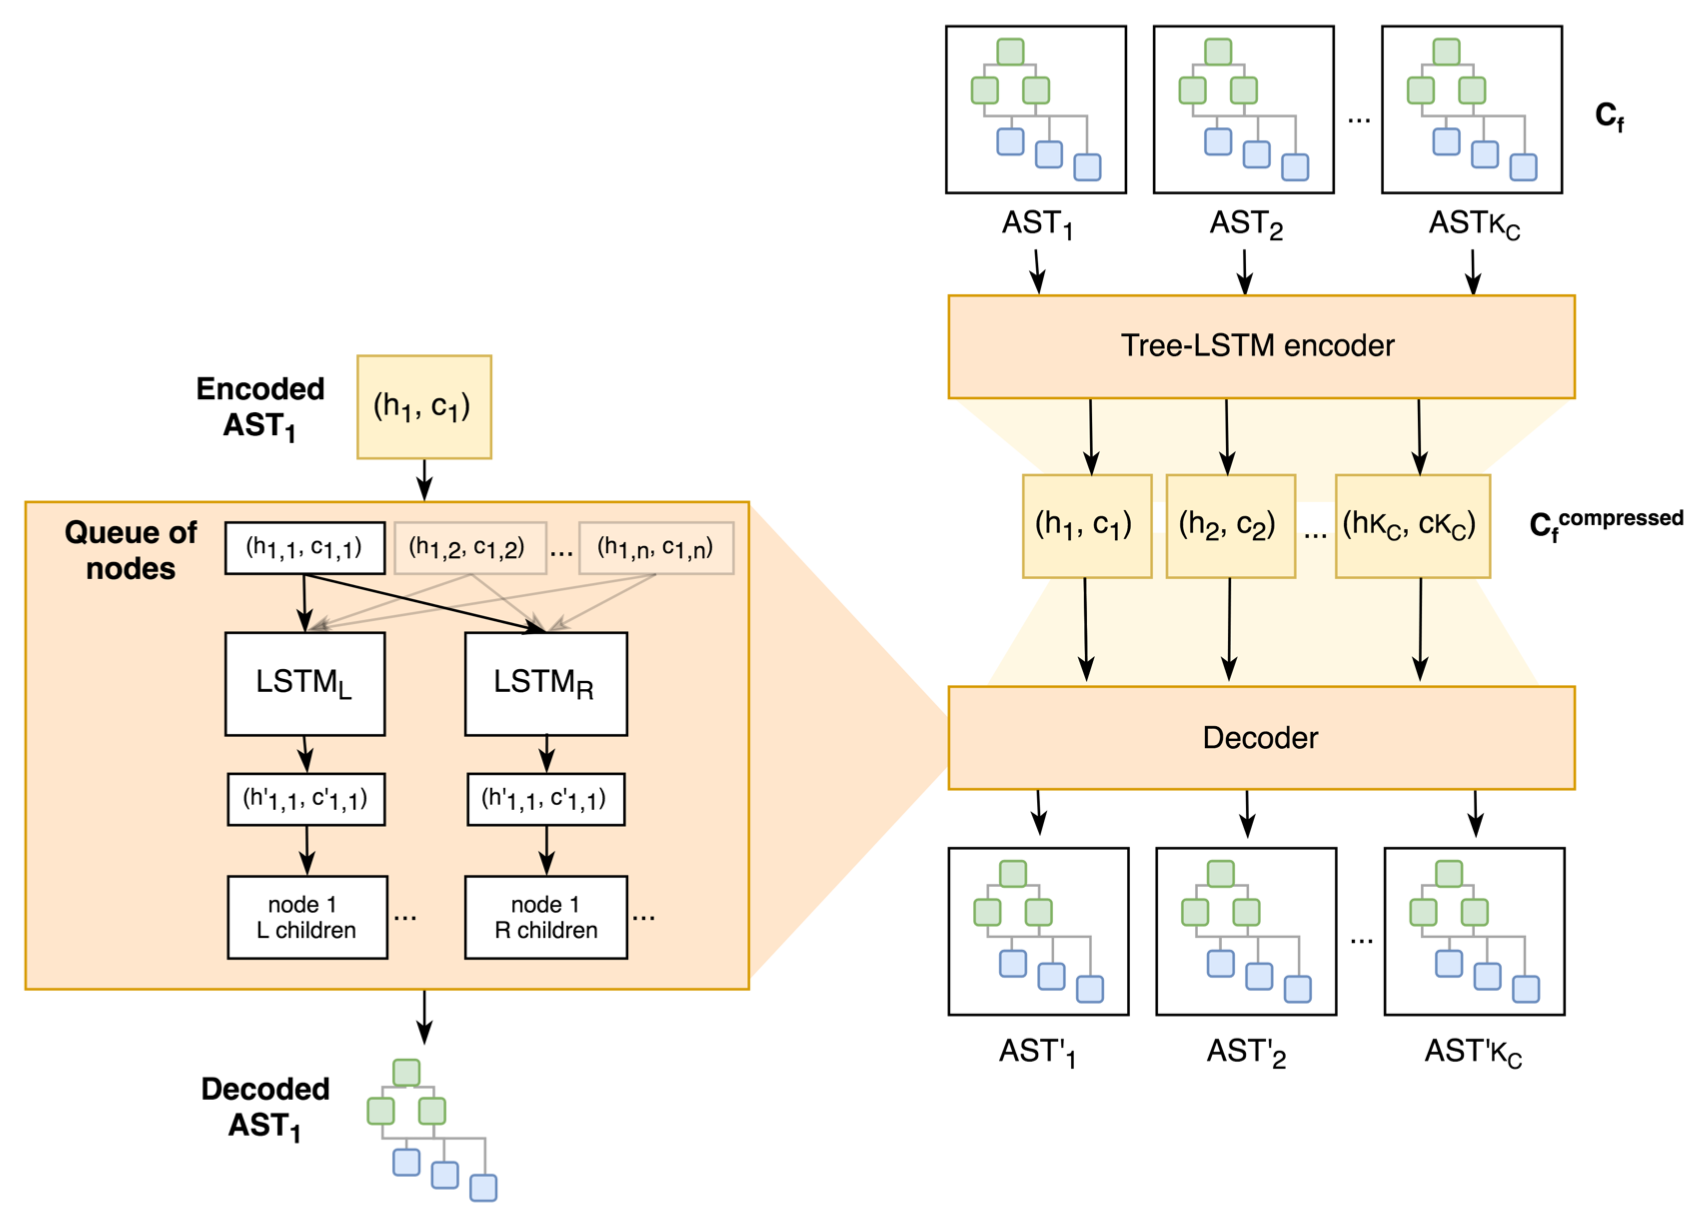
\includegraphics[width=11.0in]{./figures/CS379C_Final_Project_Gomezetal_Figure_03.png}
  \end{center}
%
  \caption{Summary of the proposed LSTM-based state-embedding architecture for $C_{f}$ \emdash{} courtesy of Gomez~\etal{}~\cite{CS379C_Final_Project_Gomezetal-18}.}
%
  \hrule{}
%
\end{figure}

%%% %%%%%%%%%%%%%%%%%%%%%%%%%%%%%%%%%%%%%%%%%%%%%%%%%%%%%%%%%%%%%%%%%%%%%%%%%%%% 

Figure~{\urlh{#fig_CS379C_Final_Project_Gomezetal_Figure_03}{3}} ... 

\subsubsectional{Resources}

Daniel Abolafia's {\urlh{https://web.stanford.edu/class/cs379c/calendar_invited_talks/lectures/04/24/slides/Daniel_Abolafia_CS379C_04-24-18.pdf}{presentation}} on iterative optimization for program synthesis in the presence of a reward function over the output of programs, where the goal is to find programs with maximal rewards~\cite{AbolafiaetalCoRR-18}\footnote{%
%
  The abstract for Abolafia~\etal{}~\cite{AbolafiaetalCoRR-18}:
%
  \begin{quotation}
%
    We consider the task of program synthesis in the presence of a reward function over the output of programs, where the goal is to find programs with maximal rewards. We employ an iterative optimization scheme, where we train an RNN on a dataset of K best programs from a priority queue of the generated programs so far. Then, we synthesize new programs and add them to the priority queue by sampling from the RNN. We benchmark our algorithm, called priority queue training (or PQT), against genetic algorithm and reinforcement learning baselines on a simple but expressive Turing complete programming language called BF. Our experimental results show that our simple PQT algorithm significantly outperforms the baselines. By adding a program length penalty to the reward function, we are able to synthesize short, human readable programs.
%
  \end{quotation}}.

Graham Neubig's {\urlh{https://web.stanford.edu/class/cs379c/calendar_invited_talks/lectures/05/01/slides/Graham_Neubig_CS379C_05-01-18.pdf}{presentation}} on a novel neural architecture for parsing natural language descriptions into source code powered by a grammar model to explicitly capture the target syntax as prior knowledge~\cite{YinandNeubigACL-17}\footnote{%
%
  The abstract for Yin and Neubig~\cite{YinandNeubigACL-17}:
%
  \begin{quotation}
%
    We consider the problem of parsing natural language descriptions into source code written in a general-purpose programming language like Python. Existing data-driven methods treat this problem as a language generation task without considering the underlying syntax of the target programming language. Informed by previous work in semantic parsing, in this paper we propose a novel neural architecture powered by a grammar model to explicitly capture the target syntax as prior knowledge. Experiments find this an effective way to scale up to generation of complex programs from natural language descriptions, achieving state-of-the-art results that well outperform previous code generation and semantic parsing approaches.
%
  \end{quotation}}.

Rishabh Singh's {\urlh{https://web.stanford.edu/class/cs379c/calendar_invited_talks/lectures/05/24/videos/Rishabh_Singh_CS379C_05-24-18.mp4}{presentation}} on using a strong statistical model for semantic code repair to predict bug locations and exact fixes without access to information about the intended correct behavior of the program.~\cite{DevlinetalICLR-18}\footnote{%
%
  The abstract for Devlin~\etal{}~\cite{DevlinetalICLR-18}:
%
  \begin{quotation}
%
    We study the problem of semantic code repair, which can be broadly defined as automatically fixing non-syntactic bugs in source code. The majority of past work in semantic code repair assumed access to unit tests against which candidate repairs could be validated. In contrast, the goal here is to develop a strong statistical model to accurately predict both bug locations and exact fixes without access to information about the intended correct behavior of the program. Achieving such a goal requires a robust contextual repair model, which we train on a large corpus of real-world source code that has been augmented with synthetically injected bugs. Our framework adopts a two-stage approach where first a large set of repair candidates are generated by rule-based processors, and then these candidates are scored by a statistical model using a novel neural network architecture which we refer to as Share, Specialize, and Compete. Specifically, the architecture (1) generates a  shared encoding of the source code using an RNN over the abstract syntax tree, (2) scores each candidate repair using specialized network modules, and (3) then normalizes these scores together so they can compete against one another in comparable probability space. We evaluate our model on a real-world test set gathered from GitHub containing four common categories of bugs. Our model is able to predict the exact correct repair 41\% of the time with a single guess, compared to 13\% accuracy for an attentional sequence-to-sequence model.
%
  \end{quotation}}.

Dawn Song and Xinyun Chen's {\urlh{https://web.stanford.edu/class/cs379c/calendar_invited_talks/lectures/05/31/videos/Dawn_Song_CS379C_05-31-18.mp4}{presentation}} on program synthesis from input-output examples, tree-to-tree neural networks for program translation, and attention for program synthesis from natural lanquage descriptions~\cite{ChenetalICLR-18b}\footnote{%
%
  The abstract for Chen~\etal{}~\cite{ChenetalICLR-18b}:
%
  \begin{quotation}
%
    Program translation is an important tool to migrate legacy code in one language into an ecosystem built in a different language. In this work, we are the first to consider employing deep neural networks toward tackling this problem. We observe that program translation is a modular procedure, in which a sub-tree of the source tree is translated into the corresponding target sub-tree at each step. To capture this intuition, we design a tree-to-tree neural network as an encoder-decoder architecture to translate a source tree into a target one. Meanwhile, we develop an attention mechanism for the tree-to-tree model, so that when the decoder expands one non-terminal in the target tree, the attention mechanism locates the corresponding sub-tree in the source tree to guide the expansion of the decoder. We evaluate the program translation capability of our tree-to-tree model against several state-of-the-art approaches. Compared against other neural translation models, we observe that our approach is consistently better than the baselines with a margin of up to 15 points. Further, our approach can improve the previous state-of-the-art program translation approaches by a margin of 20 points on the translation of real-world projects.
%
  \end{quotation}}.

%%% %%%%%%%%%%%%%%%%%%%%%%%%%%%%%%%%%%%%%%%%%%%%%%%%%%%%%%%%%%%%%%%%%%%%%%%%%%%%


